\subsection{Receiver Sensitivity and Selectivity}
\label{subsec:rx-sense-select}

When it comes to radio receivers, two of the most critical performance metrics are \textit{sensitivity} and \textit{selectivity}. These terms might sound like they belong in a psychology textbook, but in the world of radio technology, they are all about how well your receiver can pick up and distinguish signals. Let’s dive into what these terms mean and why they matter.

\subsubsection*{Sensitivity: The Art of Hearing Whispers}
Receiver sensitivity is all about how well your receiver can detect weak signals. Think of it as the receiver’s ability to hear a whisper in a noisy room. The more sensitive the receiver, the fainter the signals it can pick up. Sensitivity is typically measured in microvolts ($\mu V$) or decibels relative to one milliwatt (dBm). The lower the value, the better the sensitivity. For example, a receiver with a sensitivity of $0.1 \mu V$ can detect much weaker signals than one with a sensitivity of $1 \mu V$.

Mathematically, sensitivity can be expressed as:
\begin{equation}
    S = 10 \log_{10} \left( \frac{P_{\text{min}}}{1 \text{mW}} \right)
    \label{eq:sensitivity}
\end{equation}
where $P_{\text{min}}$ is the minimum detectable power. This equation tells us that sensitivity is a logarithmic measure of the smallest signal power the receiver can detect.


\begin{figure}[h]
    \centering
    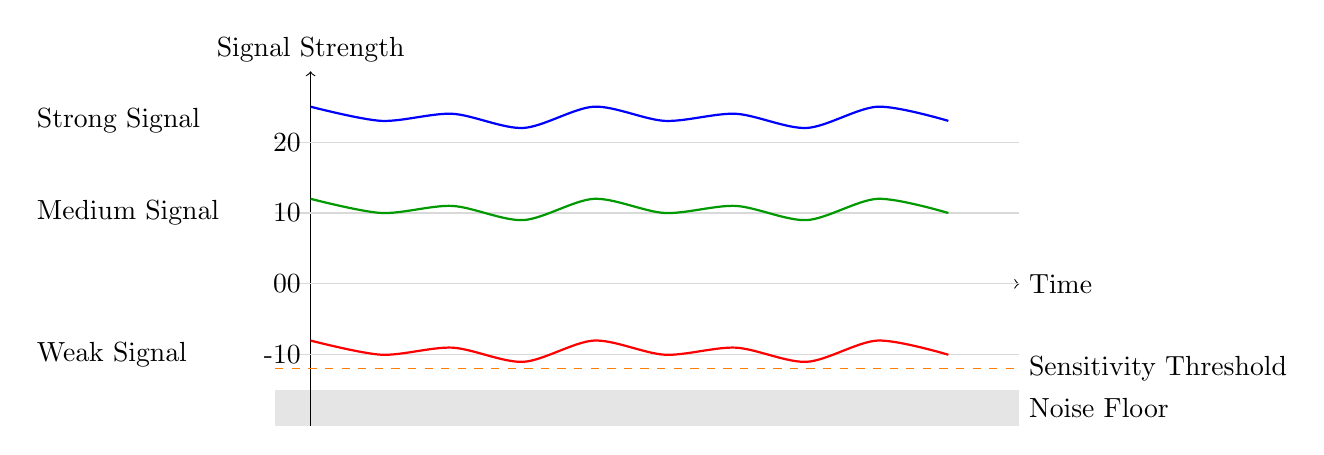
\begin{tikzpicture}[scale=0.9]
        % Define noise floor
        \fill[gray!20] (-0.5,-2) rectangle (10,-1.5);
        \node[right] at (10,-1.75) {Noise Floor};
        
        % Draw signal strength axis
        \draw[->] (-0.5,0) -- (10,0) node[right] {Time};
        \draw[->] (0,-2) -- (0,3) node[above] {Signal Strength};
        
        % Draw grid lines and labels
        \foreach \y in {-1,0,1,2} {
            \draw[gray!30] (-0.5,\y) -- (10,\y);
            \node[left] at (0,\y) {\y0};
        }
        
        % Draw three signals of different strengths
        \draw[thick,blue] plot[smooth] coordinates {
            (0,2.5) (1,2.3) (2,2.4) (3,2.2) (4,2.5) (5,2.3) (6,2.4) (7,2.2) (8,2.5) (9,2.3)
        };
        \node[right] at (-4,2.3) {Strong Signal};
        
        \draw[thick,green!60!black] plot[smooth] coordinates {
            (0,1.2) (1,1.0) (2,1.1) (3,0.9) (4,1.2) (5,1.0) (6,1.1) (7,0.9) (8,1.2) (9,1.0)
        };
        \node[right] at (-4,1.0) {Medium Signal};
        
        \draw[thick,red] plot[smooth] coordinates {
            (0,-0.8) (1,-1.0) (2,-0.9) (3,-1.1) (4,-0.8) (5,-1.0) (6,-0.9) (7,-1.1) (8,-0.8) (9,-1.0)
        };
        \node[right] at (-4,-1.0) {Weak Signal };
        
        % Draw sensitivity threshold
        \draw[dashed,orange] (-0.5,-1.2) -- (10,-1.2);
        \node[right] at (10,-1.2) {Sensitivity Threshold};
        
        
    \end{tikzpicture}
    \caption{Sensitivity in Radio Receivers: The diagram shows three signals of different strengths relative to the receiver's sensitivity threshold and noise floor. Signals must be above both the sensitivity threshold and noise floor to be detected reliably.}
    \label{fig:sensitivity-diagram}
\end{figure}

\subsubsection*{Selectivity: The Art of Ignoring Noise}
While sensitivity is about detecting weak signals, selectivity is about ignoring the ones you don’t want. Selectivity refers to the receiver’s ability to discriminate between multiple signals, especially those that are close in frequency. Imagine trying to listen to your favorite radio station while another station is broadcasting on a nearby frequency. A receiver with good selectivity can filter out the unwanted station, letting you enjoy your music without interference.

Selectivity is often measured in terms of bandwidth and rejection ratio. A narrower bandwidth generally means better selectivity, as it allows the receiver to focus on a smaller range of frequencies. The rejection ratio indicates how well the receiver can suppress signals outside its desired bandwidth.


\begin{figure}[h]
    \centering
    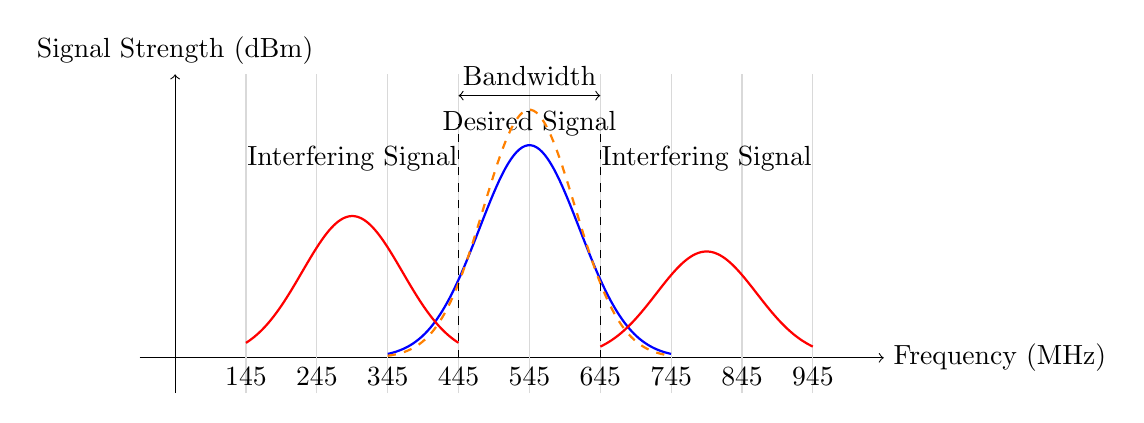
\begin{tikzpicture}[scale=0.9]
        % Draw axes
        \draw[->] (-0.5,0) -- (10,0) node[right] {Frequency (MHz)};
        \draw[->] (0,-0.5) -- (0,4) node[above] {Signal Strength (dBm)};
        
        % Draw grid lines
        \foreach \x in {1,2,3,4,5,6,7,8,9} {
            \draw[gray!30] (\x,-0.5) -- (\x,4);
            \node[below] at (\x,0) {\x45};
        }
        
        % Draw desired signal (center frequency)
        \draw[thick,blue] plot[domain=3:7,samples=100] 
            (\x,{3*exp(-(\x-5)*(\x-5))});
        \node[above] at (5,3) {Desired Signal};
        
        % Draw interfering signals
        \draw[thick,red] plot[domain=1:4,samples=100] 
            (\x,{2*exp(-(\x-2.5)*(\x-2.5))});
        \node[above] at (2.5,2.5) {Interfering Signal};
        
        \draw[thick,red] plot[domain=6:9,samples=100] 
            (\x,{1.5*exp(-(\x-7.5)*(\x-7.5))});
        \node[above] at (7.5,2.5) {Interfering Signal};
        
        % Draw selectivity filter response
        \draw[dashed,orange,thick] plot[domain=3:7,samples=100] 
            (\x,{3.5*exp(-1.2*(\x-5)*(\x-5))});
        % \node[below] at (11,2) {Filter Response};
        
        % Draw bandwidth markers
        \draw[<->] (4,3.7) -- (6,3.7) node[midway,above] {Bandwidth};
        \draw[dashed] (4,0) -- (4,3.3);
        \draw[dashed] (6,0) -- (6,3.3);
        
        % Add rejection ratio indicator
        % \draw[<->] (5,3) -- (5,0.5) node[midway,right] {Rejection Ratio};
        
        % Add explanatory text
        
    \end{tikzpicture}
    \caption{Selectivity in Radio Receivers: The diagram shows how a receiver's selectivity filter responds to signals at different frequencies. The desired signal (blue) passes through while interfering signals (red) are attenuated. The bandwidth determines the range of frequencies accepted.}
    \label{fig:selectivity-diagram}
\end{figure}

\subsubsection*{Sensitivity vs. Selectivity: A Friendly Rivalry}
While sensitivity and selectivity are both crucial for receiver performance, they often pull in opposite directions. A highly sensitive receiver might pick up weak signals, but it could also pick up more noise and interference. On the other hand, a highly selective receiver might filter out unwanted signals, but it could also miss some of the weaker ones. The key is to strike a balance between the two, depending on your specific needs.



\begin{table}[h]
    \centering
    \begin{tabular}{|l|l|l|}
        \hline
        \textbf{Parameter} & \textbf{Sensitivity} & \textbf{Selectivity} \\
        \hline
        Definition & Ability to detect weak signals & Ability to discriminate between signals \\
        \hline
        Measurement & Microvolts ($\mu V$) or dBm & Bandwidth and rejection ratio \\
        \hline
        Impact & Detects faint signals & Reduces interference \\
        \hline
    \end{tabular}
    \caption{Comparison of Sensitivity and Selectivity}
    \label{tab:sensitivity-selectivity}
\end{table}

\subsubsection*{Questions}

\begin{tcolorbox}[colback=gray!10!white,colframe=black!75!black,title={T7A01}]
    Which term describes the ability of a receiver to detect the presence of a signal?
    \begin{enumerate}[label=\Alph*),noitemsep]
        \item Linearity
        \item \textbf{Sensitivity}
        \item Selectivity
        \item Total Harmonic Distortion
    \end{enumerate}
\end{tcolorbox}

Sensitivity is the term that describes a receiver's ability to detect weak signals. It is measured in microvolts or dBm, and a lower value indicates better sensitivity. The other options, such as linearity and total harmonic distortion, are related to different aspects of receiver performance.

\begin{tcolorbox}[colback=gray!10!white,colframe=black!75!black,title={T7A04}]
    Which term describes the ability of a receiver to discriminate between multiple signals?
    \begin{enumerate}[label=\Alph*),noitemsep]
        \item Discrimination ratio
        \item Sensitivity
        \item \textbf{Selectivity}
        \item Harmonic distortion
    \end{enumerate}
\end{tcolorbox}

Selectivity is the ability of a receiver to distinguish between multiple signals, especially those close in frequency. It is crucial for reducing interference. Sensitivity, on the other hand, is about detecting weak signals, while harmonic distortion is related to signal quality.
